% Possible values for aspect ratio are: 169, 1610, 149, 54, 43 and 32.
\documentclass[aspectratio=1610]{beamer}
\usetheme{cern}

% Change bullet points
\usepackage{enumitem}
\setbeamertemplate{itemize items}[square]
\setitemize{label=\raisebox{0.3ex}{\usebeamerfont*{itemize item}
\usebeamercolor[fg]{itemize item}
\usebeamertemplate{itemize item}}}
%\setlist[itemize]{leftmargin=*, itemsep=0pt, parsep=2pt, labelsep*=2em, labelindent=0em, before=\vspace{-\dimexpr\baselineskip +2.6\partopsep}}

% CERN blue is Pantone 286 = RGB 56 97 170, defined as cern@blue below
\definecolor{cern@ltblue}{rgb}{0.415686,0.611765,0.964706} % RGB 106 156 246
\definecolor{cern@blue}  {rgb}{0.219608,0.380392,0.666667} % RGB  56  97 170
\definecolor{cern@dkblue}{rgb}{0.082353,0.184314,0.364706} % RGB  21  47  93

% Complimentary colours
\definecolor{cern@ltcomp}{rgb}{0.666667,0.525490,0.219608} % RGB 170 134  56
\definecolor{cern@dkcomp}{rgb}{0.364706,0.266667,0.047059} % RGB  93  68  12

%\setbeamercolor{title}               {bg=cern@blue,fg=white}
%\setbeamercolor{frametitle}          {bg=cern@blue,fg=white}
%\setbeamercolor{section in head/foot}{bg=cern@ltblue,fg=white}
\setbeamercolor{itemize item}         {fg=cern@dkcomp}
\setbeamerfont{itemize item}          {size=\large}



%%
%% Get packages that we need
%%

% Adjust page margins on-the-fly
\usepackage{changepage}

% Change fonts to Avenir
% Note: need to compile with xelatex to use this package
\usepackage{fontspec}
\setsansfont{AvenirLTStd-Book}

\usepackage[showboxes,overlay,absolute]{textpos}
\usepackage[overlay,absolute]{textpos}
\setlength{\TPHorizModule}{.01\paperwidth} % Horizontal units are percent of paper width
\setlength{\TPVertModule}{.01\paperwidth}  % Make vertical units equal to horizontal units
\textblockorigin{.5\paperwidth}{4.25ex}

% Headings within slides
\usepackage{xcolor}
\usepackage{tabularx}



%%
%% Title page
%%

\author{\Large Michael Davis}
\title[CTA Deployment and Migration]{CERN Tape Archive (CTA) :\\
Deployment and Migration from CASTOR\\}
\date{11 December 2019}

\begin{document}

\frame{\titlepage}

\begin{frame}{EOS+CTA Overview}
\begin{itemize}
   \item CTA is the tape back-end to EOS
   % Main difference with CASTOR: EOSCTA is a pure tape system.
   % Disk cache duty consolidated in main EOS instance.
   \item EOS+CTA offers the ``Best of Both Worlds''
   \begin{itemize}
       \item User interface and file access from EOS
       \item Tape system management from CASTOR
       \item New scalable, robust queuing system to link the two
   \end{itemize}
   \item CTA design principles
   \begin{itemize}
      \item Simplicity
      \item Scalabilty
      \item Performance
   \end{itemize}
\end{itemize}
\end{frame}

\begin{frame}{EOS+CTA Performance Enhancements}
   Reduced latency compared to CASTOR
\begin{itemize}
   \item Just-in-time scheduling
   \item Preemptive scheduling\\[2ex]
\end{itemize}
   New features for Run--3
\begin{itemize}
   \item Recommended Access Order (RAO) for LTO media
   \item Colocation hints
\end{itemize}
\end{frame}

\begin{frame}{EOS+CTA Architecture}
  \centering
   \includegraphics<1>[width=0.6\textwidth]{images/arch_CASTOR}
   \includegraphics<2>[width=0.6\textwidth]{images/arch_CTA}
\end{frame}

\begin{frame}{EOS+CTA Architecture}
  \centering
  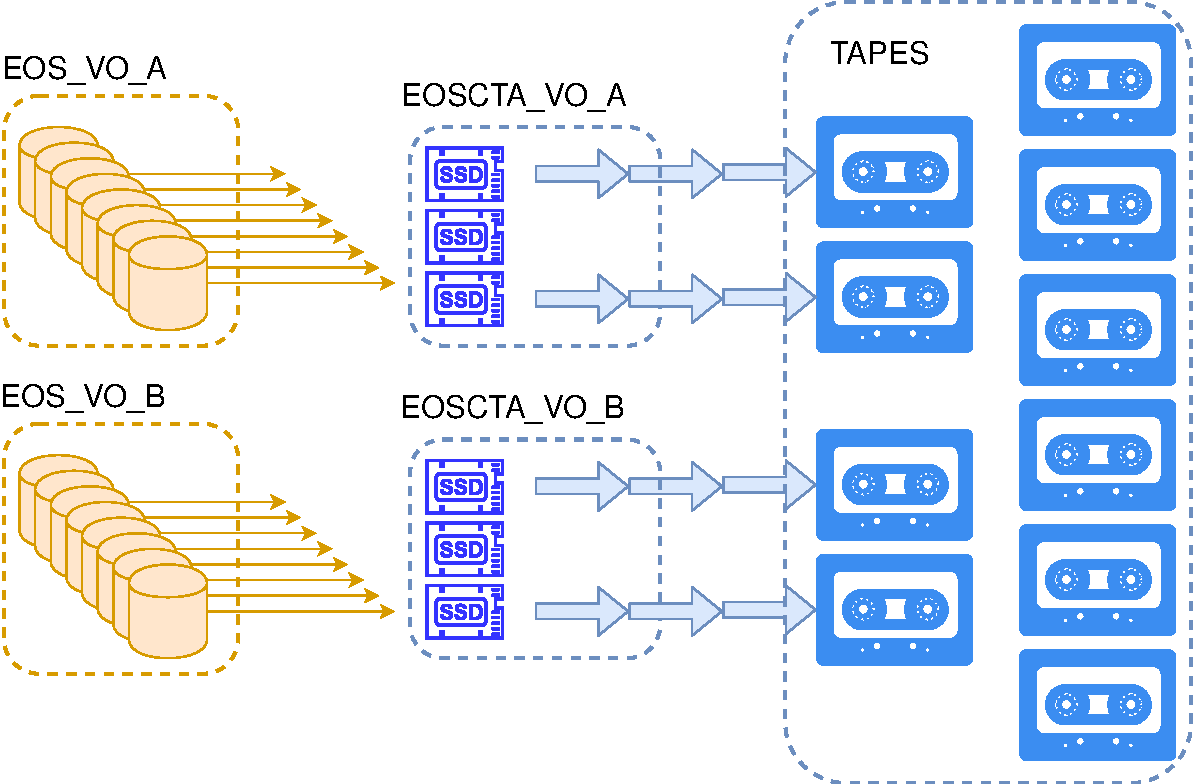
\includegraphics[width=0.7\textwidth]{images/upload_e764d94a4ee3ac79c328ea0d21a6a128.pdf}
\end{frame}

\begin{frame}{EOS+CTA Deployment}
   \begin{itemize}
      \item 4 instances for the LHC experiments
      \item 1 instance for PUBLIC
      \begin{itemize}
         \item Active non-LHC experiments: \textit{AMS, Compass, Dune, NA61, NA62, nTOF, \ldots}
         \item Inactive legacy experiments: \textit{LEP, \ldots}
         \item CASTOR backup
         \item User files
      \end{itemize}
   \item Tier-1s: \textit{RAL}
   \end{itemize}
\end{frame}

\begin{frame}{EOS+CTA Timeline}
  \centering
  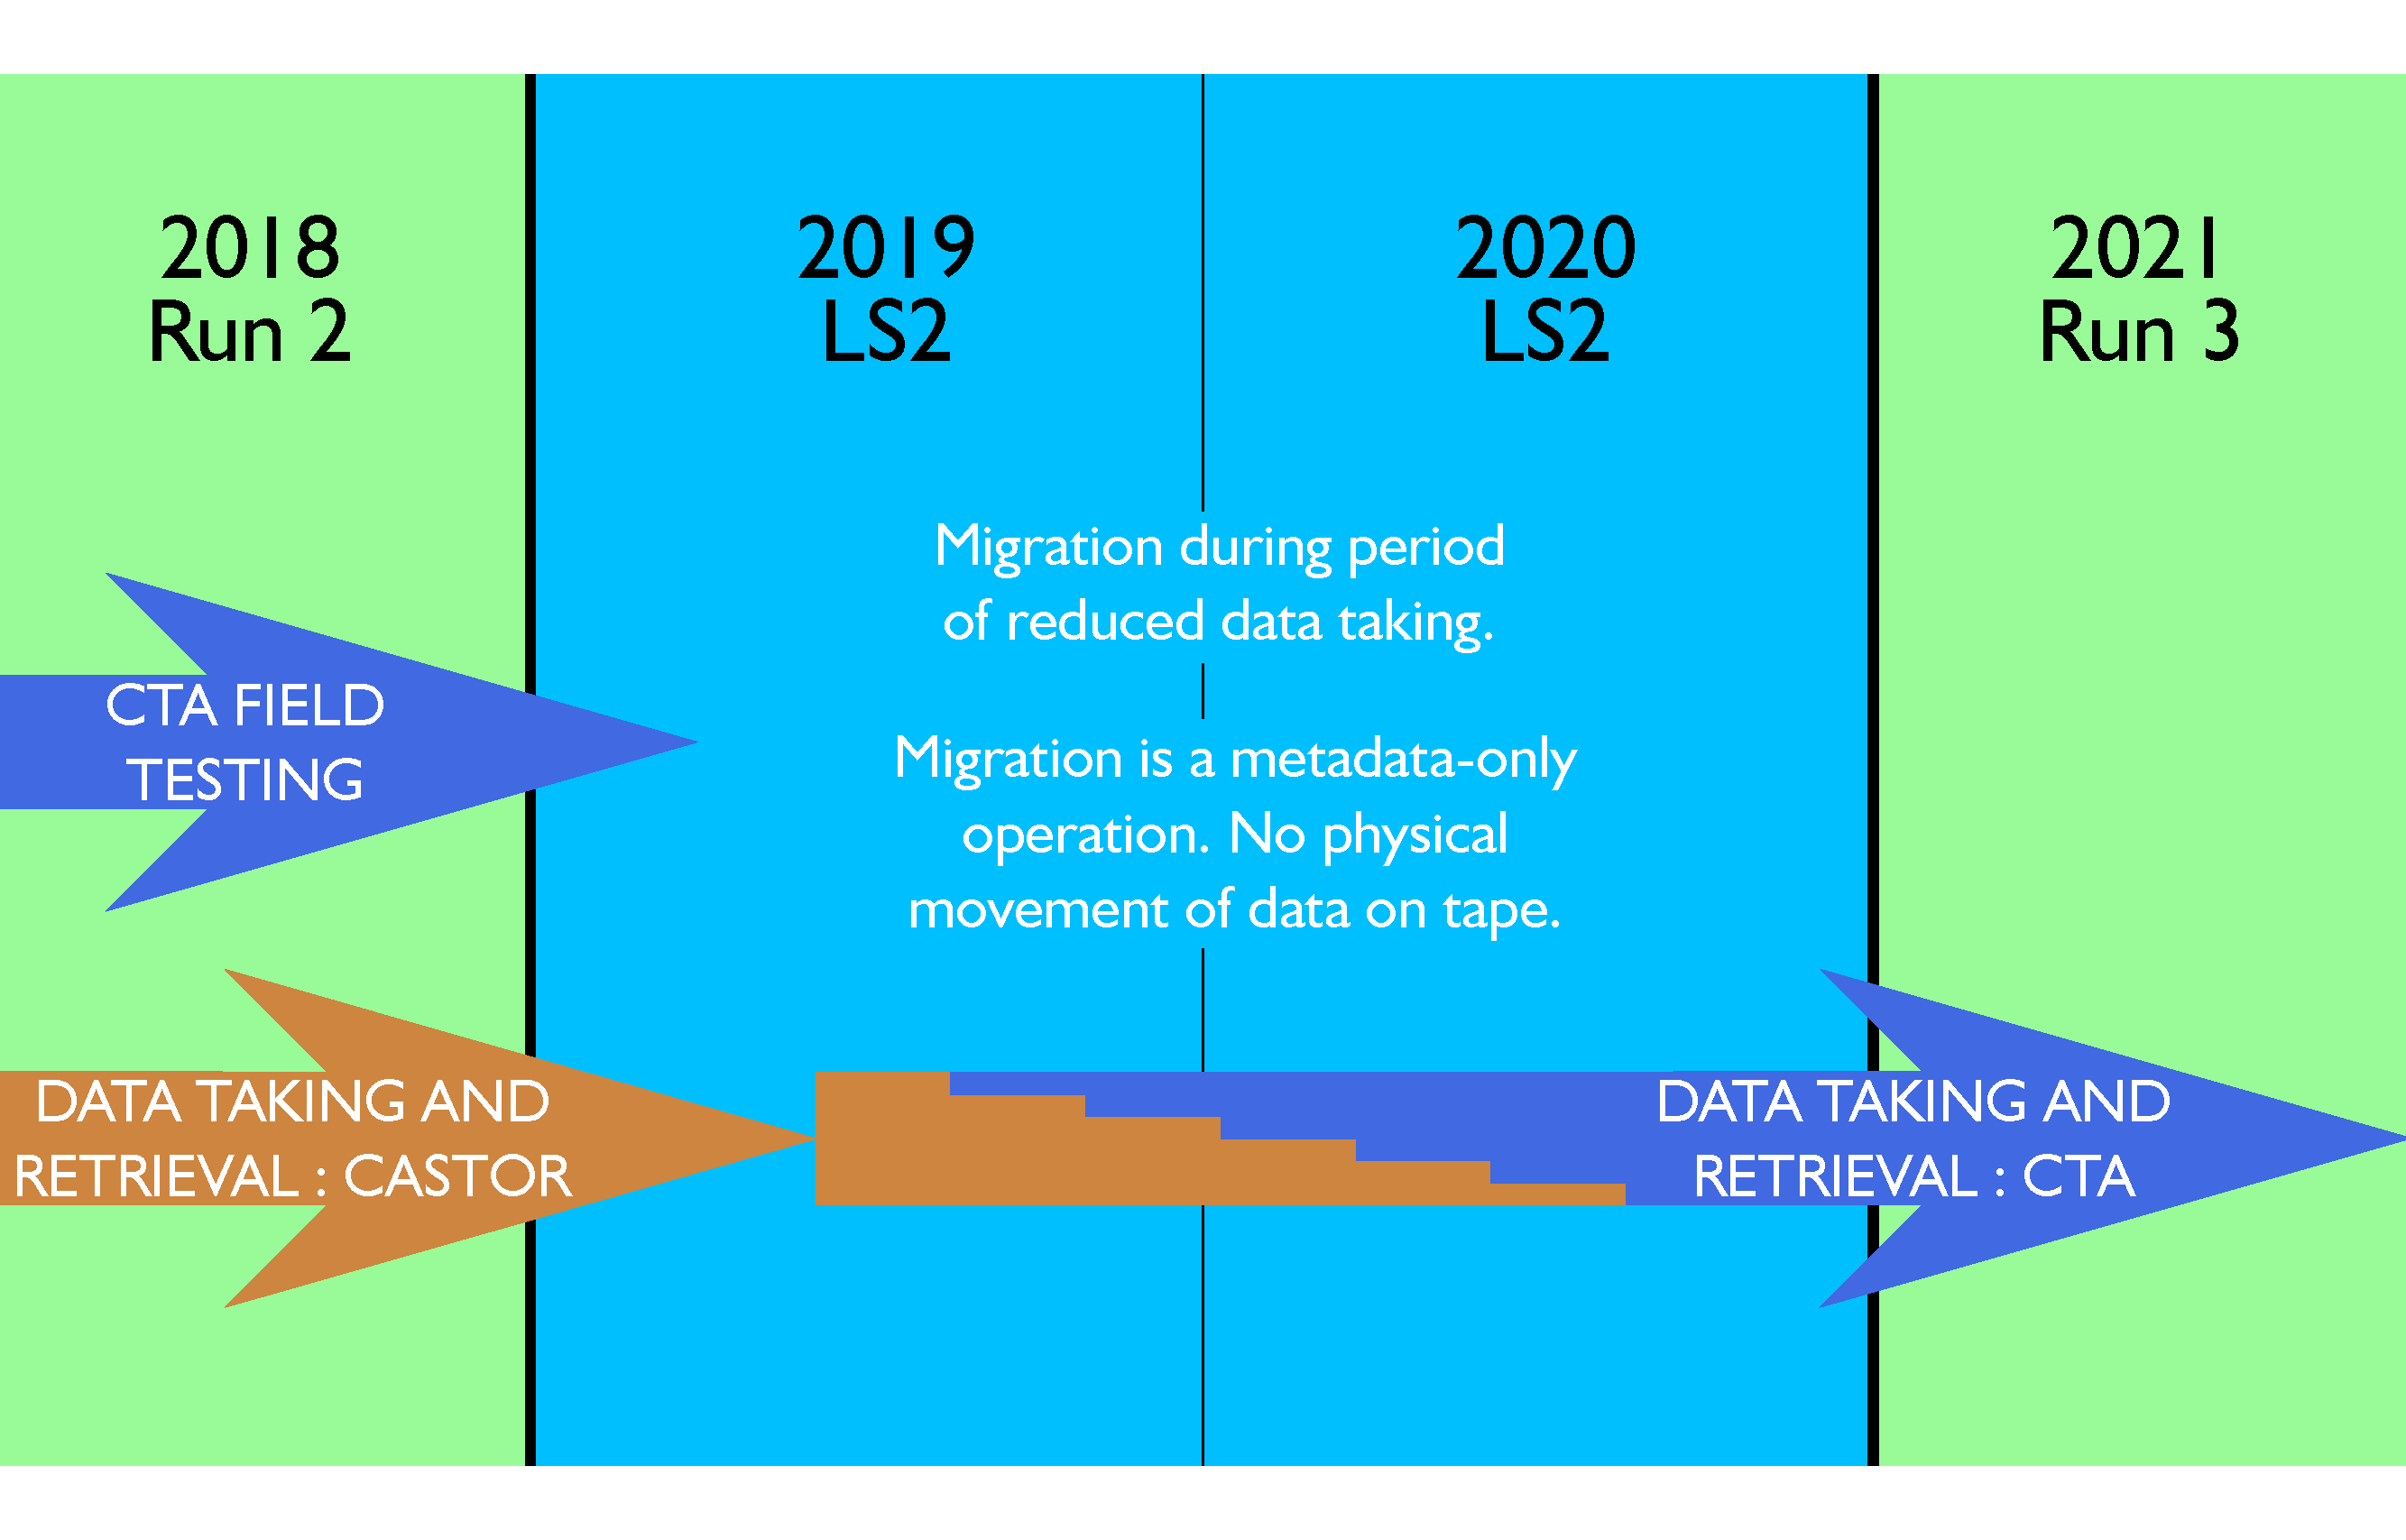
\includegraphics[width=0.85\textwidth]{images/upload_0ae96233cb49710754263e2d780a20b6.pdf}
\end{frame}

\begin{frame}{EOS+CTA Status: Hardware}
   \begin{itemize}
      \item Racks are cabled
      \item Network switches are allocated (6$\times$ 100 Gb/s links)
      \item 32$\times$ hyper-converged servers have been delivered to CERN.
         Operating tape drive at full-speed, full-time requires SSD-based buffer.
      \begin{itemize}
         \item 16$\times$ 1.92 TB SSD
         \item 25 Gb/s Ethernet
      \end{itemize}
   \end{itemize}
% 24x 2.5" hot-swappable SSD slots
% 2x Intel Xeon Scalable 5218 processors
% 192GB of DDR4 ECC Reg memory running at 2667 MHz (M393A2K43BB1-CTD)
% 1x 512GB Samsung 970 EVO Plus NVMe SSD for OS (MZ-V7P512BW)
% 16x 1.92TB Intel S4510 SSD (SSDSC2KB019T801) running firmware >= XCV10110
% 2x 25Gbit/s Ethernet ports and 1x dedicated management port
\end{frame}

\begin{frame}{Max. throughput, minimum contention}
  \centering
  \vspace{1ex}
  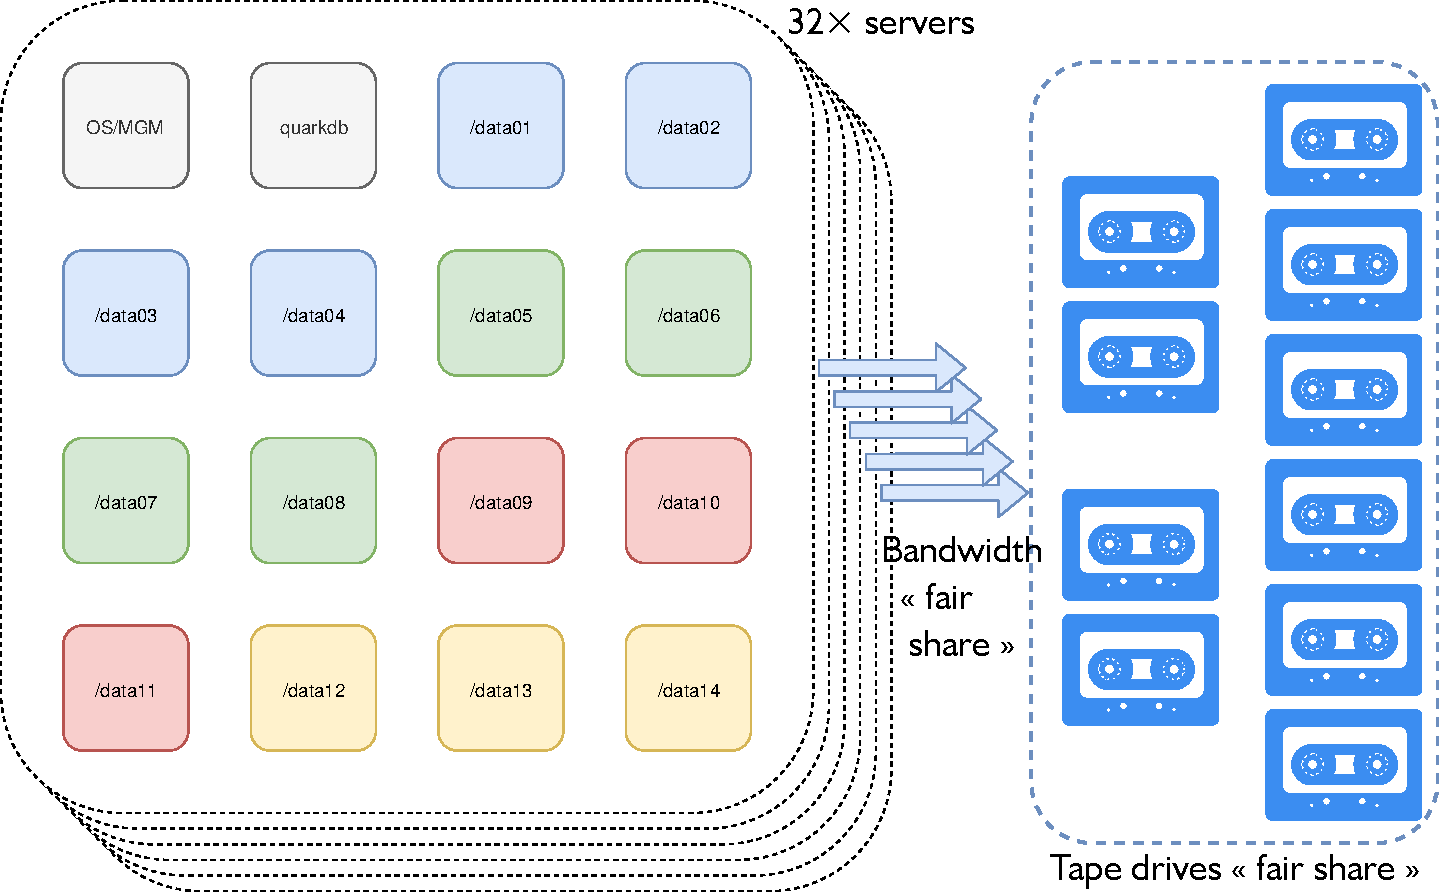
\includegraphics[width=0.8\textwidth]{images/hw_setup.pdf}
  % 7 tape libraries
  % 83 tape drives
  % 30K tapes
\end{frame}

\begin{frame}{EOS+CTA Status: Software}
   \begin{itemize}
      \item CTA v1.0 release 11 December
      \item Workflows have been integrated with FTS and Rucio (via XRootD)
      \item Deployment onto production instances as soon as hardware is ready
   \end{itemize}
\end{frame}

\begin{frame}{Commissioning (January 2020)}
   \begin{itemize}
      \item Migrate CASTOR ATLAS to CTA ATLAS ($\approx$90 million files, read-only copy)
      \item 4--5 servers dedicated to ATLAS to offer 10 GB/s
      \item ATLAS Run--2 reprocessing campaign
   \begin{itemize}
      \item Targetting 3--4 PB from CTA (out of 18 PB total)
   \end{itemize}
      \item ATLAS data taking stress test
   \end{itemize}
\end{frame}

\begin{frame}{ATLAS Migration (1Q 2020)}
   Schedule to be agreed with ATLAS, contingent on successful reprocessing campaign

   \begin{itemize}
      \small
      \item Disable the tapes in CASTOR
      \item Extract metadata
      \begin{itemize}
         \item CASTOR Catalogue $\rightarrow$ CTA Catalogue
         \item CASTOR Namespace $\rightarrow$ EOS Namespace ($\approx$ 6 million files per hour)
      \end{itemize}
      \item Enable tapes in CTA
      \item Rucio: update all CASTOR endpoints to CTA
   \end{itemize}

   Risk Mitigation

   \begin{itemize}
      \small
         \item CTA is prohibited from writing to tapes imported from CASTOR
         \item To return a tape to CASTOR, disable the tape in the CTA catalogue and re-enable the tape in CASTOR
   \end{itemize}
\end{frame}

\begin{frame}{ALICE Migration (2Q 2020)}
\begin{columns}
	\begin{column}{0.4\textwidth}
		\begin{center}
		  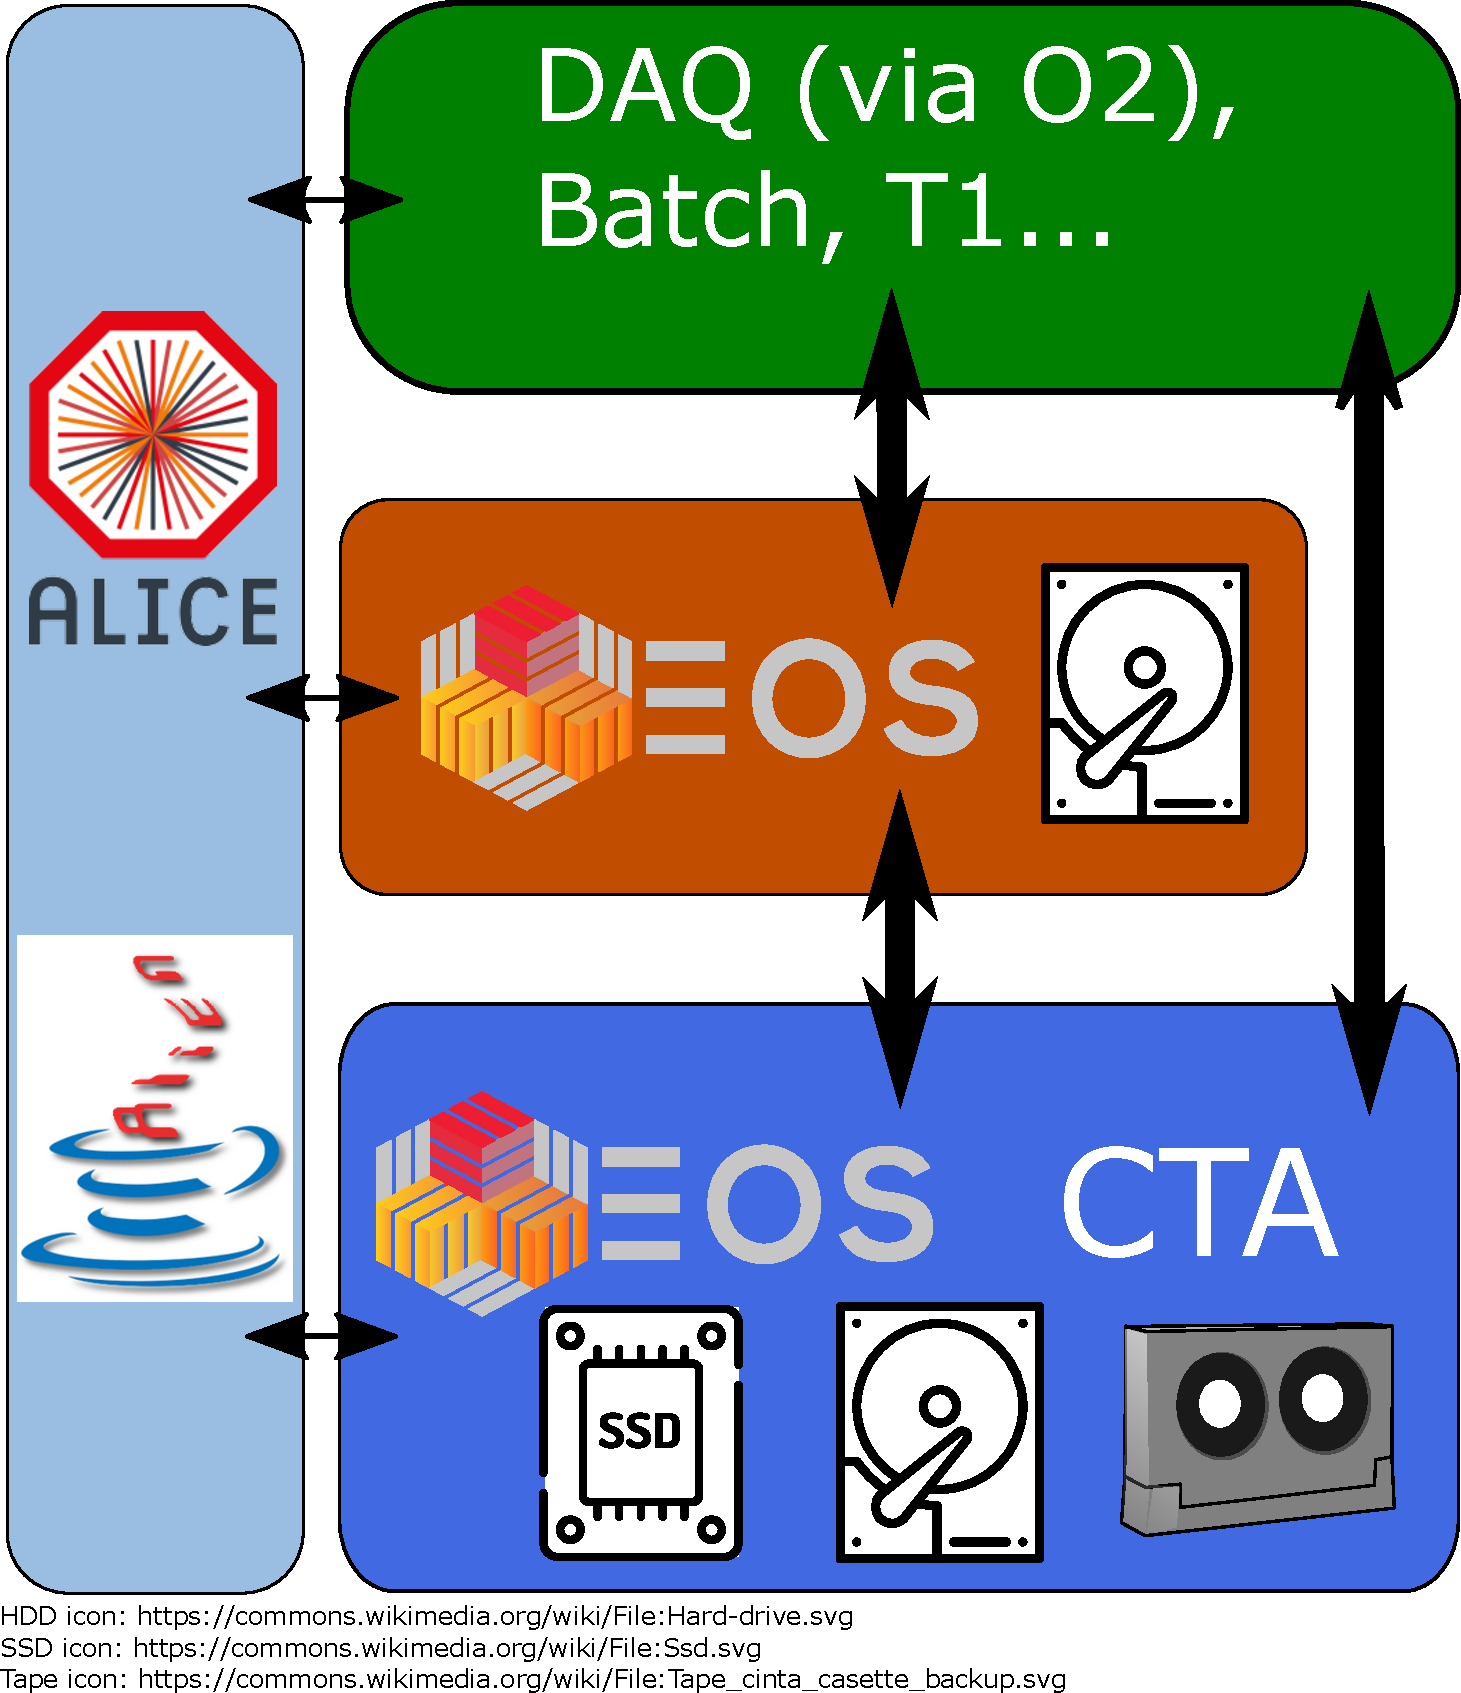
\includegraphics[width=\textwidth]{images/CTA_Deployment_ALICE.pdf}
		\end{center}
	\end{column}
	\begin{column}{0.55\textwidth}
      Schedule to be agreed with ALICE\\[1ex]

      Integration with JAlien:
		\begin{itemize}
         \item Dual Space buffer
		\begin{itemize}
		  \item SSD buffer for data taking
		  \item $\approx$5 PB HDD cache for retrieves, with garbage collection
		\end{itemize}
		  \item Requirement for occasional T1 access to EOSCTA
		\end{itemize}
	\end{column}
\end{columns}
\end{frame}

\begin{frame}{CMS Migration (2H 2020)}
\begin{columns}
	\begin{column}{0.4\textwidth}
		\begin{center}
		  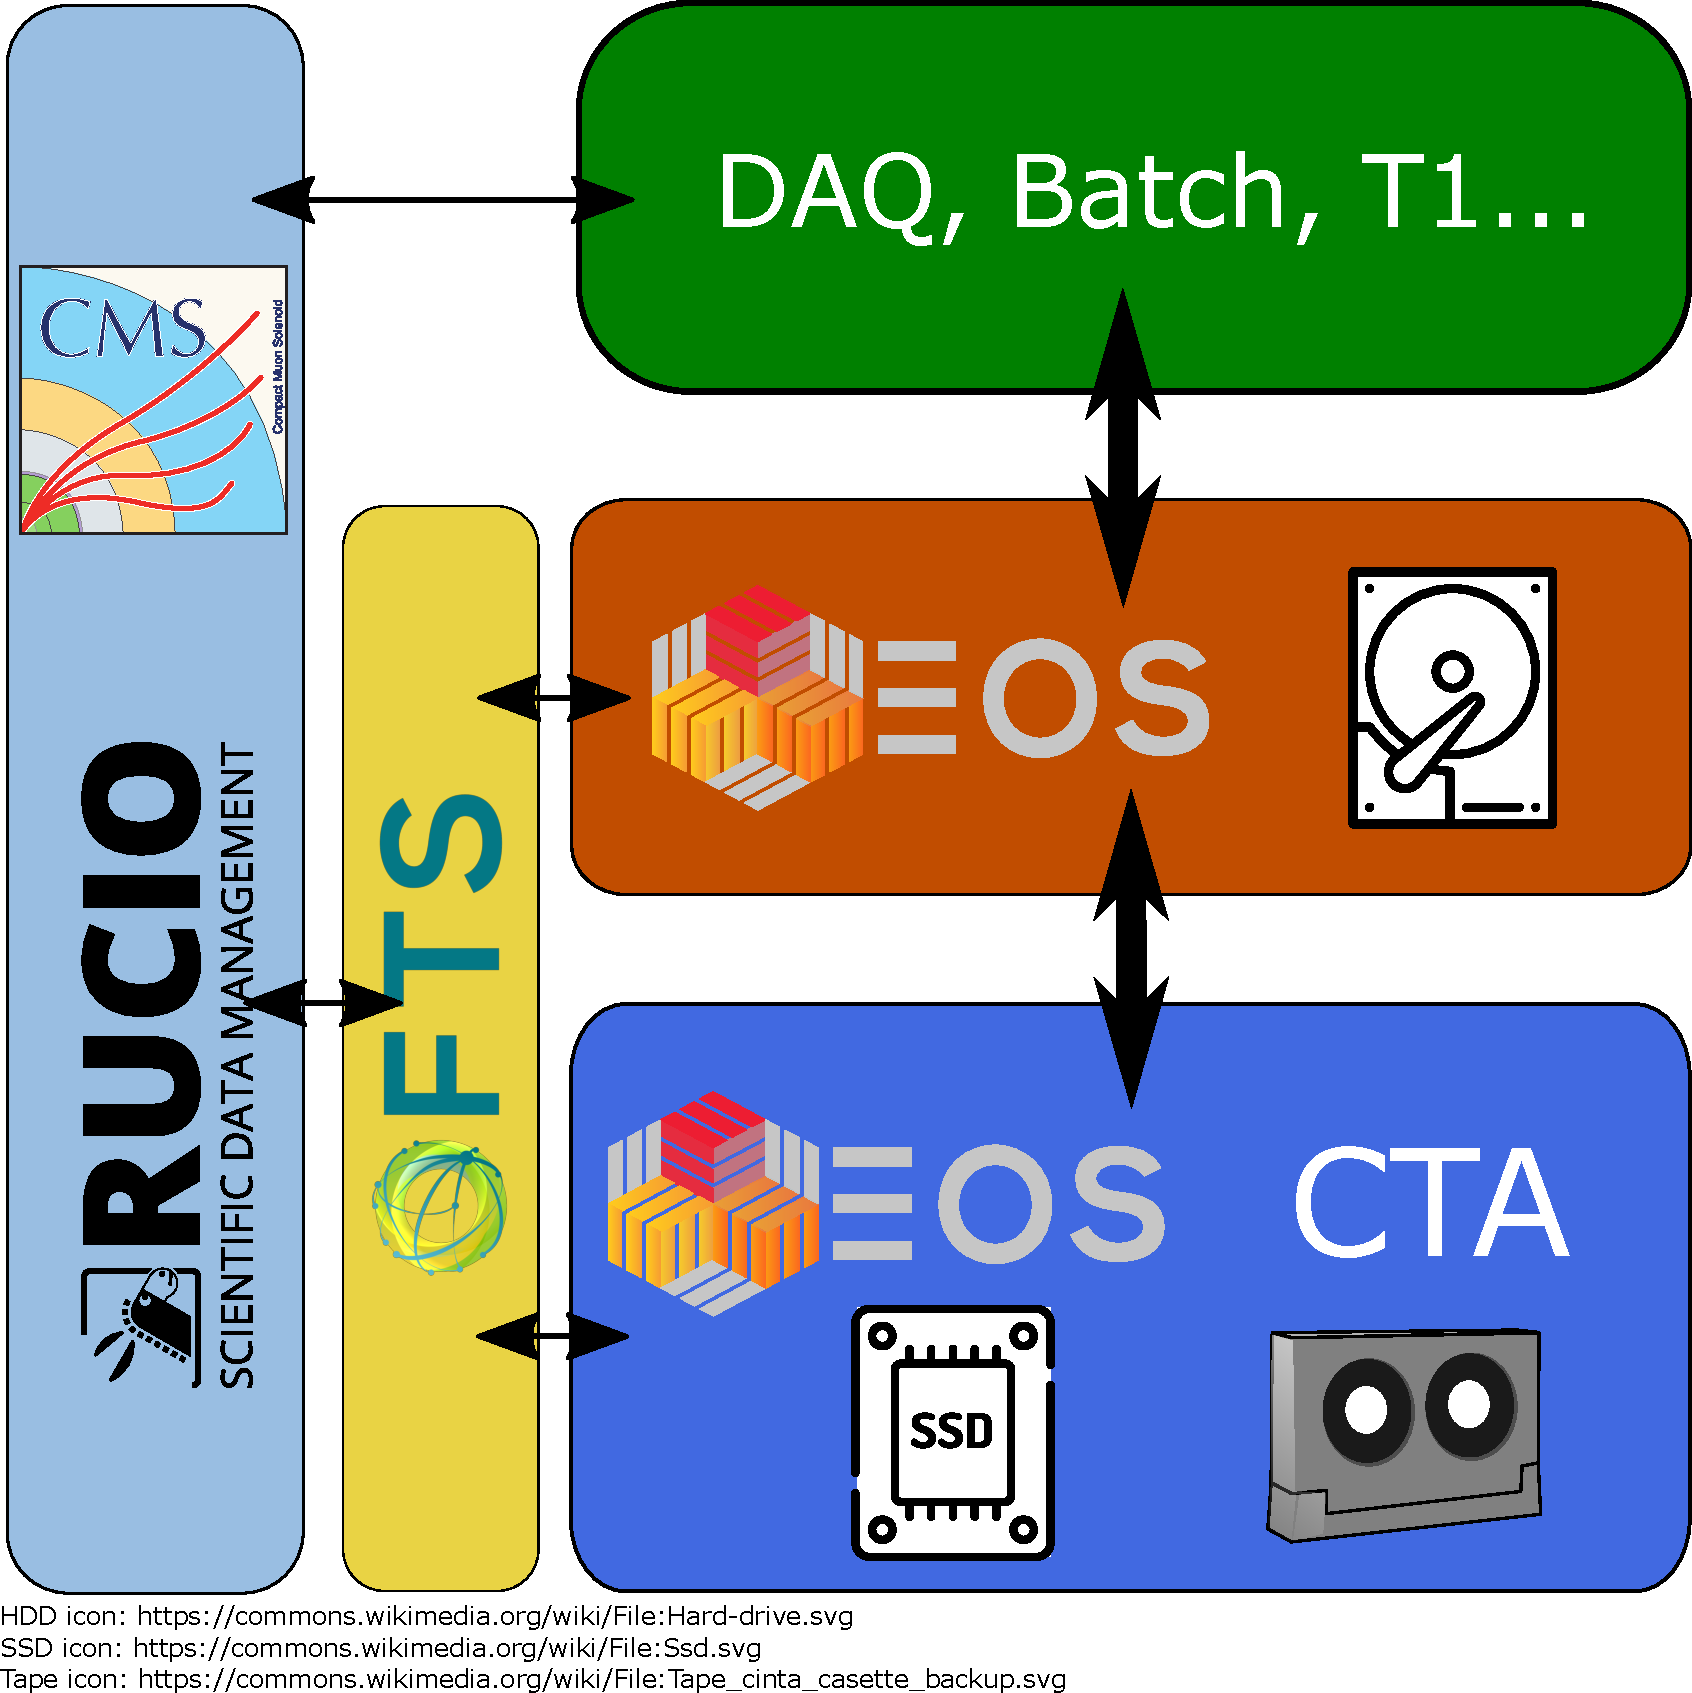
\includegraphics[width=\textwidth]{images/CTA_Deployment_CMS.pdf}
		\end{center}
	\end{column}
	\begin{column}{0.55\textwidth}
		\begin{itemize}
		  \item Similar setup to ATLAS : Rucio + FTS + EOSCTA
        \item Schedule driven by CMS adoption of Rucio
		\end{itemize}
	\end{column}
\end{columns}
\end{frame}

\begin{frame}{LHCb Migration (2H 2020)}
\begin{columns}
	\begin{column}{0.4\textwidth}
		\begin{center}
		  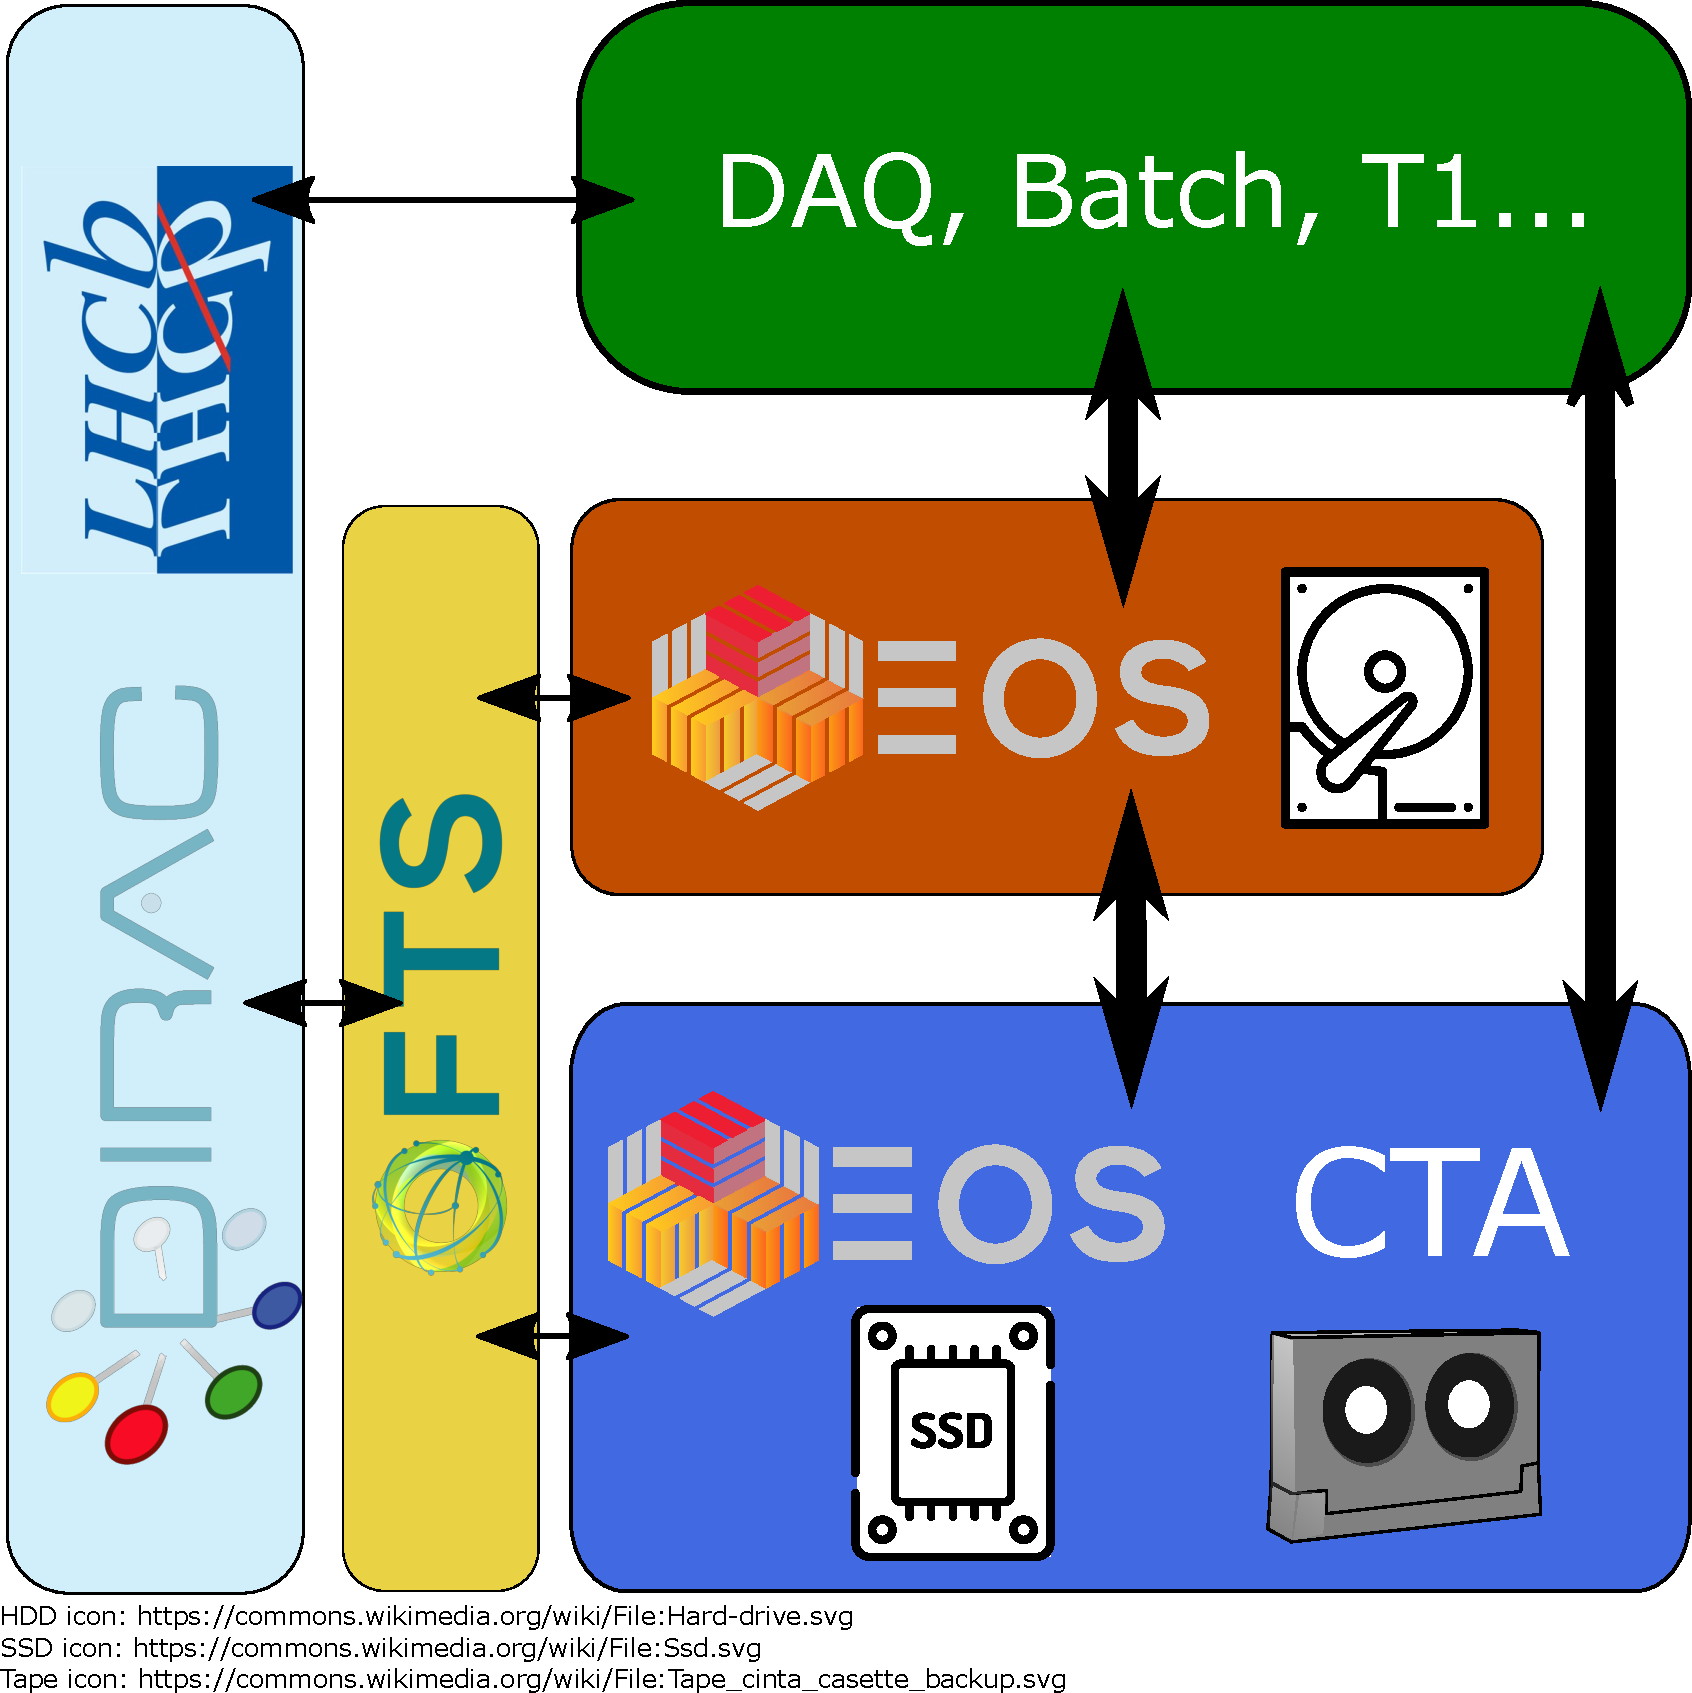
\includegraphics[width=\textwidth]{images/CTA_Deployment_LHCb.pdf}
		\end{center}
	\end{column}
	\begin{column}{0.55\textwidth}
		\begin{itemize}
		  \item Similar setup to ATLAS and CMS : Dirac + FTS + EOSCTA
		  \item Requirement for occasional export from EOSCTA to T1
        \item Schedule driven by T1s supporting XRootD 3rd Party Copy with delegation
		\end{itemize}
	\end{column}
\end{columns}
\end{frame}

\begin{frame}{EOS+CTA Status: Summary}
\begin{itemize}
    \item Hardware to be installed by end of year
    \item Software to be deployed by end of year
    \item January 2020: Stress testing and commissioning (ATLAS)
    \item 1Q 2020: ATLAS migration CASTOR $\rightarrow$ EOS+CTA
    \item 2Q 2020: ALICE testing and migration CASTOR $\rightarrow$ EOS+CTA
    \item Other LHC experiments to be migrated before YE 2020
\end{itemize}
\end{frame}

\backcover

\end{document}
